\section{Improved robot arm mechanical design (L.~Hofland and R.~Carroll}
\label{sec:robotarmmechanical}

The preliminary design concept did not have a well accepted robot arm / snipper / gripper concept for taking and retaining the sample. As a result, in Spring 2020, the team brainstormed and developed futher concepts for the robot arm / snipper / gripper and backed them up with prototype testing, including a ``lawnmower'' (propeller snoot chopper), a ``guillotine'' nonchopping snoot, a pip3 arm, and a buzzsaw concept. The buzzsaw concept was recommended for further development. 

\begin{enumerate}
\item Telescoping razor blades:
\begin{figure}
\begin{center}
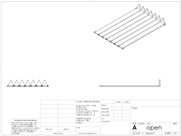
\includegraphics[height=1.5in]{figures/robotarmmech1a.png}
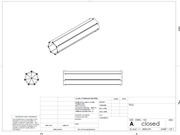
\includegraphics[height=1.5in]{figures/robotarmmech1b.png}
\end{center}
\end{figure}
\begin{enumerate}
\item Pros: snips and grips with one fluid motion
\item Cons: complex, hard to build
\item Primary failure: unreliable cut and likely blade failure
\item Design Rejected
\end{enumerate}

\item Bladed jaw
\begin{figure}
\begin{center}
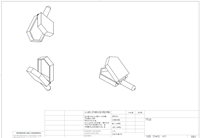
\includegraphics[height=1.5in]{figures/robotarmmech2a.png}
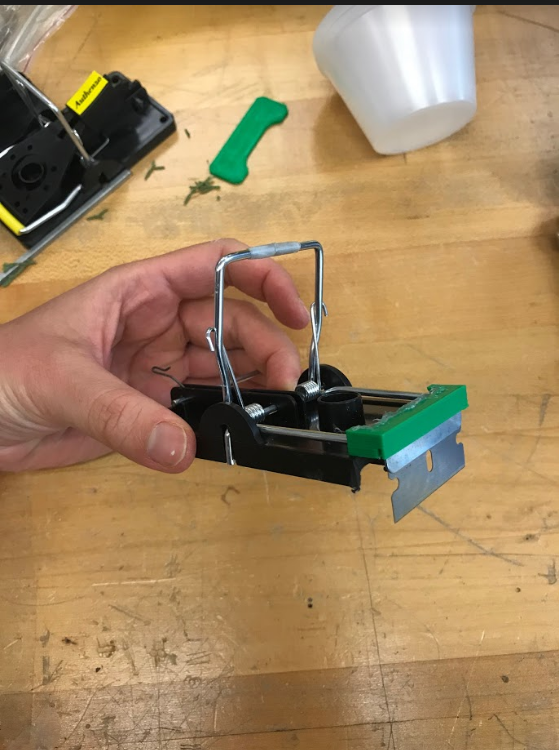
\includegraphics[height=1.5in]{figures/robotarmmech2b.png}
\end{center}
\end{figure}
\begin{enumerate}
\item Pros: simplified design
\item Primary failure: unable to cut catastrophic blade failure during testing.
\item Design Rejected
\item Notes: design powered by a mousetrap
\end{enumerate} 

\item Automated Pruning shears
\begin{figure}
\begin{center}
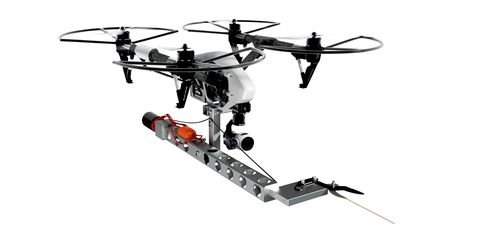
\includegraphics[height=1.5in]{figures/robotarmmech3.png}
\end{center}
\end{figure}
\begin{enumerate}
\item Pros: verified cutting capability under ideal conditions
\item Cons: complex, heavy
\item Primary failure: Gipping design difficult
\item Design Rejected
\end{enumerate}

\item Cigar Cutter
\begin{figure}
\begin{center}
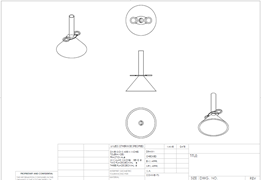
\includegraphics[height=1.5in]{figures/robotarmmech4a.png}
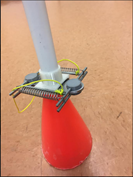
\includegraphics[height=1.5in]{figures/robotarmmech4b.png}
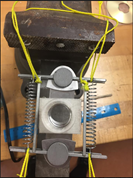
\includegraphics[height=1.5in]{figures/robotarmmech4c.png}
\end{center}
\end{figure}
\begin{enumerate} 
\item Pros: successful test of both snipping and gripping. Simple design, easily operated, lightweight
\item Primary failure: One shot one kill
\item Design Rejected
\end{enumerate}

\item Propeller snoot chopper
\begin{enumerate}
\item Pros: controllable, simple, lightweight, snipping and gripping take place simultaneously.   
\item Primary failure: Sample is blended; for botanical voucher specimen use, intact leaves, fruits, and flowers are desired. Blended samples also risk mixing DNA. 
\item Design Rejected
\end{enumerate}

\item Nonchopping snoot
\begin{figure}
\begin{center}
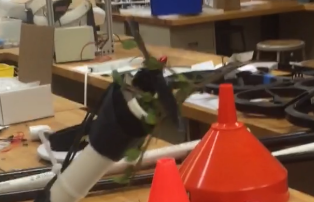
\includegraphics[height=1.5in]{figures/robotarmmech6.png}
\end{center}
\end{figure}
\begin{enumerate}
\item Pros: Sample is not blended
\item Primary failure: After testing this design failed to snip even a small branch
\item Design Rejected
\end{enumerate}

\item Pipe Arm
\begin{figure}
\begin{center}
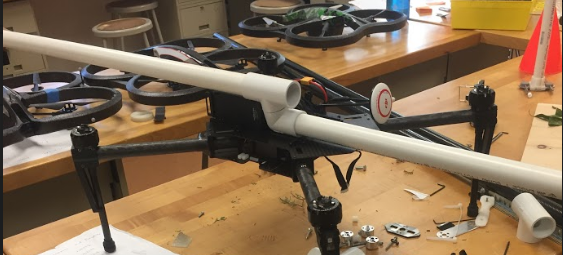
\includegraphics[height=1.5in]{figures/robotarmmech7.png}
\end{center}
\end{figure}
\begin{enumerate}
\item Lightweight, functional, balanced
\item Primary failure: design rejected in favor of controllable robotic arm. 
\end{enumerate}

\item Buzzsaw arm grabber
\begin{figure}
\begin{center}
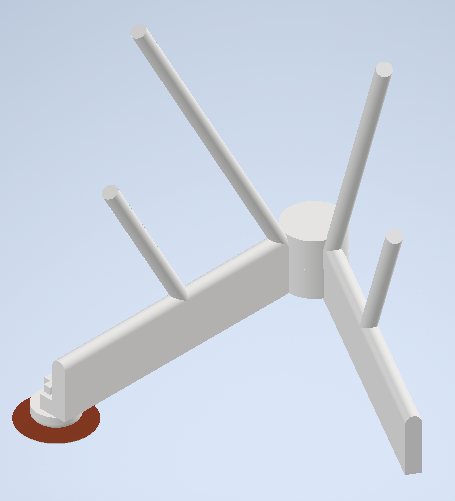
\includegraphics[height=1.5in]{figures/robotarmmech8.png}
\end{center}
\end{figure}
\begin{enumerate}
\item Pros: Controllable, lightweight, captures samples in one piece
\item Mounted on the end of a robotic arm. 
\item The cutting blade attached to a propeller engine
\item Lightweight netting is strung between the``fingers'' of each ``hand'' to capture the sample.
\item Current snipper/gripper design 
\end{enumerate}
\end{enumerate}
